\documentclass{article}

%\usepackage{corl_2022} % Use this for the initial submission.
%\usepackage[final]{corl_2022} % Uncomment for the camera-ready ``final'' version.
\usepackage[preprint]{corl_2022} % Uncomment for pre-prints (e.g., arxiv); This is like ``final'', but will remove the CORL footnote.
\usepackage{graphicx}

\title{STEAL: Simultaneous Trajectory Estimation And Learning \vspace{-1.5em}}

% The \author macro works with any number of authors. There are two
% commands used to separate the names and addresses of multiple
% authors: \And and \AND.
%
% Using \And between authors leaves it to LaTeX to determine where to
% break the lines. Using \AND forces a line break at that point. So,
% if LaTeX puts 3 of 4 authors names on the first line, and the last
% on the second line, try using \AND instead of \And before the third
% author name.

% NOTE: authors will be visible only in the camera-ready and preprint versions (i.e., when using the option 'final' or 'preprint'). 
% 	For the initial submission the authors will be anonymized.

\author{
  Team 11\\
  CS 7648\\
  Georgia Institute of Technology
  United States\\
  \texttt{\{varunagrawal,ssingh794,yahn41\}@gatech.edu} \\
  %% examples of more authors
  %% \And
  %% Coauthor \\
  %% Affiliation \\
  %% Address \\
  %% \texttt{email} \\
  %% \AND
  %% Coauthor \\
  %% Affiliation \\
  %% Address \\
  %% \texttt{email} \\
  %% \And
  %% Coauthor \\
  %% Affiliation \\
  %% Address \\
  %% \texttt{email} \\
  %% \And
  %% Coauthor \\
  %% Affiliation \\
  %% Address \\
  %% \texttt{email} \\
}

\setlength{\marginparwidth}{0pt}

\begin{document}
\maketitle

\vspace{-3.5em}
\section{Problem}

% We wish to learn from demonstrations in nonlinear, non-Euclidean spaces since our world is inherently nonlinear, while also accounting for suboptimality and personalization.

In order for robots to be more accessible to non-experts, they should be able to learn from multiple, potentially sub-optimal demonstrations, instead of relying on a single nominal expert trajectory. This learning should also be compatible with our inherently nonlinear world.  We propose a method for handling multiple nonlinear trajectories while accounting for sub-optimality and personalization.

%===============================================================================
\vspace{-1em}
\section{Project Motivation}

Existing works in LfD don't explicitly consider the nonlinear, non-Euclidean nature of trajectories and our physical world. Even when they do~\cite{Rana20corl}, they only operate on a single expert trajectory (obtained e.g. via Dynamic Time Warping), losing personalization and robustness to sub-optimality.
This motivates our use of RMPFlow as the motion policy generator since it can handle generic non-Euclidean spaces (or Riemannian Manifolds).

% The current approach used by RMPFlow requires the use of a single, nominal trajectory without mechanisms to handle sub-optimality. Dynamic Time Warping is used to find the nominal trajectory which in turn fully governs the learning dynamics. However, we would like to make our system robust to sub-optimal demonstrations.

Gaussian Process Regression has a number of desirable properties which motivates its use in this project. It is computationally efficient, works extremely well in the low-data regime, and can model continuous-time signals. Moreover, by defining appropriate covariance functions (either by hand or by learning it with a deep network), we automatically gain interpretability which is useful for non-expert debugging. This leads to good performance with low cognitive load for non-expert users.

%===============================================================================
\section{Approach}
% \textit{How your approach will work (or what your experiment will do to answer a novel question)?}

To be able to operate in nonlinear, non-Euclidean task spaces, we use RMPFlow for learning a controller $\pi(t; \theta)$ from demonstrations. This also grants us theoretical guarantees about safety, stability, local reactivity, and extensibility, all of which are useful in Human-Robot Interaction, while being agnostic to the robot and task type.

To incorporate multiple trajectories and be robust to sub-optimality, we leverage the use of Gaussian Processes (GPs)~\cite{Mukadam18ijrr,Bhardwaj20icra,vanWaveren22manuscript} which are a common representation for continuous-time robot trajectories. GPs use Bayesian inference to incorporate multiple trajectories as samples of a mean trajectory function, and the covariance matrix $\mathcal{K}$ helps define properties of the trajectories. The choice of $\mathcal{K}$ is a hyperparameter which allows us to incorporate personalization metrics.


%===============================================================================

\section{Project Update}

% \textit{What progress you have made since your proposal?}

\begin{itemize}
    \item Met multiple times in order to read and learn about RMPFlow and Gaussian Processes (common \& state-of-the-art techniques which are beyond the scope of the class).
    \item Baseline RMPFlow model working for simple LASA~\cite{Khansari-Zadeh11tro} dataset drawing task.
    \item GP regression (using GPyTorch) on LASA drawing task.
\end{itemize}

%===============================================================================

\section{Future Plan}

% \textit{What is your plan moving forward (including a Gantt chart)?}

\begin{itemize}
    \item Integrate the Gaussian Process representation with RMPFlow.
    \item Demonstrate end-to-end results on the LASA dataset.
    \item Collect data from Assistive Gym~\cite{Erickson20icra}.
    \item Demonstrate results on Assistive Gym dataset.
    \item Prepare 3 Ps: plots, presentation, paper.
\end{itemize}

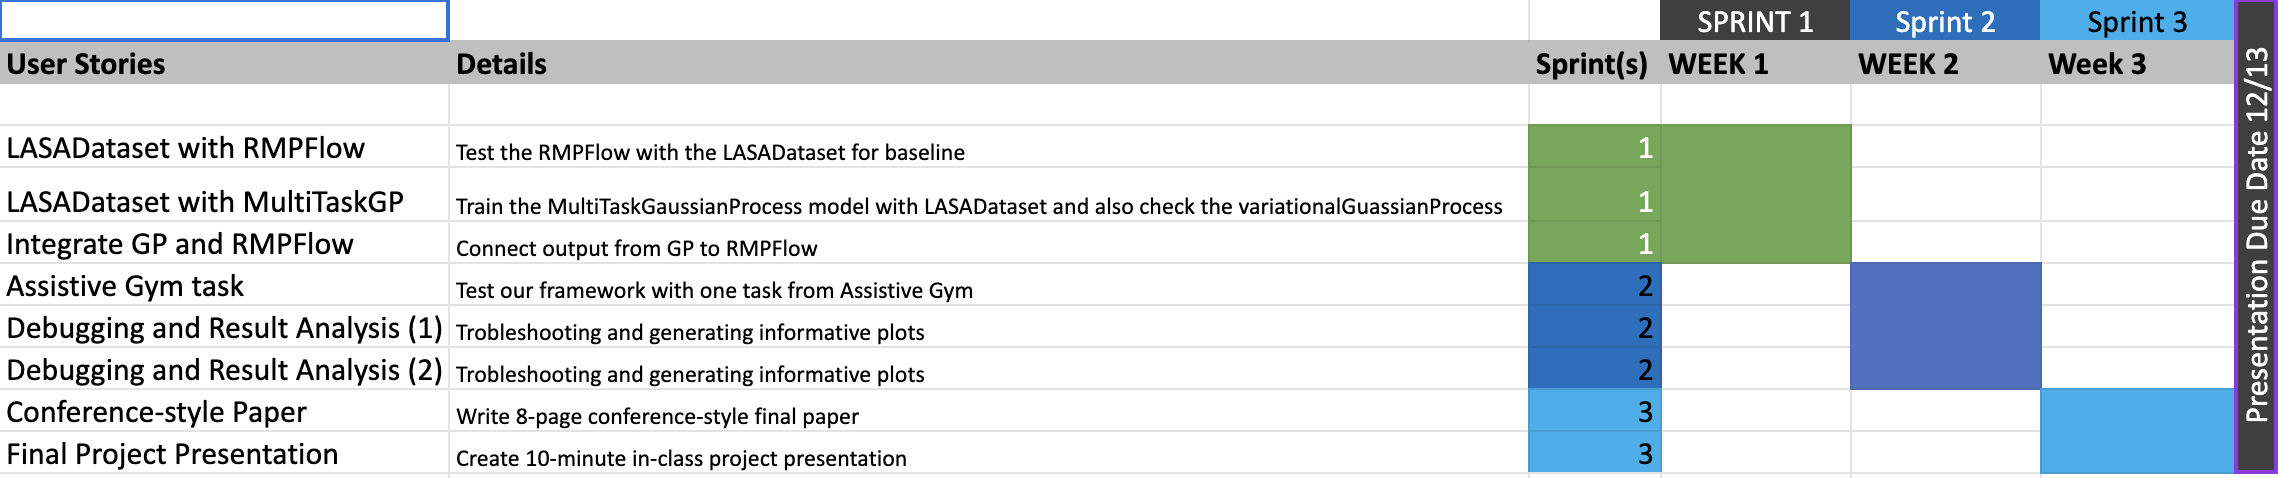
\includegraphics[width=\textwidth,bb=0 0 1000 220]{images/gantt_chart.png}

%===============================================================================

\section{Request for Feedback}

% 7) What are the major issues/questions you need my help with.
\begin{itemize}
    \item How do we present advanced topics such as RMPFlow and GPs better?
    \item What can be done additionally to make this project publication quality?
\end{itemize}
%===============================================================================

\section{Risks}
\begin{itemize}
    \item Time requirements to finish the project.
    \item Demonstrating the theoretical properties of our approach in practice.
    \item Potential unforeseen issues (e.g. Varun's visa situation).
\end{itemize}

% \section{Timeline}
% \begin{itemize}
%     \item Week 1 Setup all the necessary software. - Done!
%     \item Week 2 Data collection for push task and Assistive Gym task. - Kinda done since we got the LASA dataset. Assistive Gym is missing.
%     \item Week 3 Project design and implementation. - Done and implementationin progress.
%     \item Week 4-6 Evaluation and debugging.
%     \item Week 7 Report and presentation creation.
% \end{itemize}

%\clearpage
% The acknowledgments are automatically included only in the final and preprint versions of the paper.
%\acknowledgments{If a paper is accepted, the final camera-ready version will (and probably should) include acknowledgments. All acknowledgments go at the end of the paper, including thanks to reviewers who gave useful comments, to colleagues who contributed to the ideas, and to funding agencies and corporate sponsors that provided financial support.}

%===============================================================================

% no \bibliographystyle is required, since the corl style is automatically used.
\bibliography{refs}  % .bib

\end{document}